%\documentclass{article}
%\usepackage[a4paper, total={6in, 8in}]{geometry}
%\documentclass[reprint,amsmath,amssymb,rmp,onecolumn,notitlepage,11pt]{revtex4-1}
\documentclass[
reprint,
twocolumn,
%preprint
%onecolumn,
amsmath,amssymb,superscriptaddress,aps,
pre]{revtex4-1}
\usepackage[utf8]{inputenc}
%\usepackage{authblk}
%\usepackage{natbib}
\usepackage[normalem]{ulem}
\usepackage{graphicx}
\usepackage{hyperref}
\usepackage{xcolor}
\newcommand{\red}[1]{\textcolor{red!80!black}{#1}}
\newcommand{\blue}[1]{\textcolor{blue!80!black}{#1}}
\newcommand{\green}[1]{\textcolor{green!70!black}{#1}}
\newcommand{\gray}[1]{\textcolor{gray!80!black}{#1}}
\usepackage{mathtools}
\DeclarePairedDelimiter{\evdel}{\langle}{\rangle}
\usepackage[colorinlistoftodos]{todonotes}
\newcommand{\Pin}{P_{\mathrm{in}}}
\newcommand{\fhigh}{f_{\mathrm{high}}}
\newcommand{\flow}{f_{\mathrm{low}}}

\begin{document}
\title{Chain separation distribution in protein contact networks}
\title{Theoretical approximation of chain separation distribution in protein contact networks}
\title{Theory of chain separation distributions gives insights in real protein contact networks}
%\title{}
\author{Nora Molkenthin}
\affiliation{Potsdam Institut für Klimafolgenforschung}
\affiliation{Center for Advancing Electronics Dresden (cfaed), Technical University of Dresden}
\author{J. J.  Güven}
\affiliation{EaStCHEM School of Chemistry, University of Edinburgh, Edinburgh, United Kingdom}
\author{Steffen Mühle}
\affiliation{Max-Planck Institute for Dynamics and Self-Organization, 37077 Göttingen, Germany}
\author{Antonia S J S Mey}
\email[Author to whom correspondence should be addressed:]{antonia.mey@ed.ac.uk}
\affiliation{EaStCHEM School of Chemistry, University of Edinburgh, Edinburgh, United Kingdom}

\begin{abstract}
The mechanisms by which we can determine a protein's 3D structure based on its amino acid sequence have long been one of the key mysteries of biophysics. With the advent of AlphaFold~2, making predictions for protein structures based on amino acid sequences at an accuracy similar to experiments is now possible, yet requires a lot of available structural data for training the model. Predicting contact maps from sequence \textit{de novo} is an appealing alternative. Here, we are interested in understanding the emergent behavior of protein contact maps derived from a network ensemble perspective of a geometrically constrained random interaction model. We show that the frequency distributions of amino acid distances obtained from simulations of the geometrically constrained interaction model can be described by an analytical approximation of the two-dimensional analogue of this model. To this end, we look at the scaling behavior of the simulation with the analytical approximation for different chain lengths typically found in proteins with good agreement. Furthermore, we compare our constrained model with frequency distributions of amino acid distances from contact maps of real proteins---from the protein data bank and AlphaFold~2 database---showing that these follow a similar trend as the geometrically constrained model.   
 We therefore suggest the conclusion that the approximate power-law behavior of the amino acid distance distribution can be attributed to geometric constraints of protein chains and amino acid sequences only play a secondary role.  
%The distribution of chain separations of interacting amino acids in proteins roughly follows a power law. Here we show, analytically and in simulations, that a geometrical stochastic model of folding chains can explain this behavior. 
\end{abstract}
\maketitle

\section{Introduction}
Proteins, the molecular machines of every living organism perform vital tasks required for life to persist, ranging from transport (e.g. hemoglobin)~\cite{ahmed2020hemoglobin}, signal transduction (e.g. rhodopsin)~\cite{nagata2021rhodopsins}, immune responses (e.g. antibodies), and hormonal regulation (e.g. insulin)~\cite{dill2008protein,Dill1042}. All natural proteins are made of 20 different amino acids which dictate the three-dimensional conformations the proteins adopt in order to function~\cite{scheraga2007proteinfolding}. One of the great challenges has been to understand how the primary structure, the amino acid sequence, can lead to the fully folded functional protein. The last 50 years has seen many different routes to computationally predict biologically active protein structures without having to solve a crystal structure of the protein. [input information from Rohan's presentation]. AlphaFold~2, a machine learning model for structure prediction, has shown predictiveness at a level of experimental accuracy in the most recent protein structure prediction challenge~\cite{jumper2021highly, kryshtafovych2021critical}. This has led to an explosion of available structural protein models beyond the protein database, containing structures from crystallographic, NMR, and cryo-EM experiments~\cite{berman2000protein}. Beyond the prediction of structure understanding emergent patterns in proteins on a more fundamental level is of interest, as it opens up a deeper understanding of proteins structure and function relationship.  One way of looking at the functional forms of proteins and classifying their structural properties is by looking at protein contact maps (PCM) or protein contact networks (PCN)~\cite{Vendruscolo2002,dipaola2013protein,Estrada2011}. A PCM---we will use PCMs in favor of PCN in this paper---is the resulting adjacency matrix of spatially close amino acids, given a certain cut-off as determined typically from a protein structure. PCMs have shown promise in understanding protein folding patterns as well as revealing allosteric communication pathways~\cite{yao2019establishing, menichetti2016network,dokholyan2002topological}. Their use is also prominently featured in machine learning approaches. One challenge is to predict a PCM \textit{de novo} from sequence alone~\cite{bassot2019using, rives2021biological, rao2021msa}, without using structural data as part of the training set, as was done for AlphaFold~2. These PCMs can then be used in e.g. graph convolutional machine learning approaches to train a model able to predict binding affinities for certain types of proteins~\cite{jiang2020drug},
From a physicist's perspective it is interesting to understand the emergent behavior in protein structure by looking at PCMs. Since a PCM is an adjacency matrix and therefore a graph, it is possible to investigate PCMs using common network measures. For example, Bartoli \textit{et al.}~\cite{bartoli2008effecta} build a model in which they assume that proteins have an amino acid distance distribution that follows $s^{-1}$, where $s$ is the separation of two connected amino acids along the backbone chain (in the following called \emph{amino acid distance}) as the simplest implementation of a connection probability, thus decreasing with the distance along the sequence. However, they do not provide a quantitative explanation for this assumption. 

Here, we show how a simple geometrical model can reproduce this heuristically found behavior well, and even provide a simple analytical approximation. The three-dimensional geometrical model and the analytical approximation of its two-dimensional analogue both build on the idea that inherently geometrical objects, such as amino acids, imply that any resulting PCM network ensemble modelling them has to be spatially embedded~\cite{molkenthin2016scaling, molkenthin2020self}. 
Different approaches have been used in the past for geometrical models describing protein folding, some of which derived characteristics of the secondary structure from constraints on bond and torsion angles~\cite{bhattacharjee2013flory,Danielsson2010,Molkenthin2011} and others focused on the formation mechanisms of the tertiary structure~\cite{molkenthin2016scaling, molkenthin2020self}. 

Based on such considerations, the network formation process repeatedly connects random pairs of units, without causing any intersections along the chain~\cite{molkenthin2016scaling}. Such a model can now be used to investigate the emergent behavior of amino acid distance distributions as used heuristically by Bartoli \textit{et al.}~\cite{bartoli2008effecta}. To this end, we define and analyze the amino acid distance distributions $P(s)$ that emerge from the geometric model, where the \emph{amino acid distance} $s$ of a link is defined as the distance of the two end units along the original chain. This distribution is then compared to the amino acid distance distribution extracted from protein contact networks generated from protein data bank and AlphaFold~2 data. 

We find that, despite the highly simplified model, the generated amino acid distance distribution is in agreement with the one observed in networks generated from PDB data and roughly consistent with the heuristic $s^{-1}$ finding. The analytical approximation provides a correction term on top of the $s^{-1}$ heuristic.

%%%%%%%%%%%%%%%%%
% Section       %
%%%%%%%%%%%%%%%%%
\section{Protein contact maps}
\label{sec:methods}
The complex interaction pattern between the amino acids in a protein can be very naturally expressed as a network or graph, in which each amino acid is represented by a node and spatial proximity is encoded as a link. Whenever two central $C_\alpha$ atoms are closer together than a threshold $d_c$, they are connected, linked, or in `close contact'. These connections can be determined from the 3D functional or folded structure of the protein and are encoded in a so-called contact map. This contact map is effectively an adjacency matrix $\textbf{A}^{\mathrm{struc}}$ or binary matrix
\begin{equation}
  A^{\mathrm{struc}}_{ij}=
  \begin{cases}
   0, & \text{ if } d_{i,j}>d_c \text{ or } i=j\\
      1, & \text{ if } d_{i,j}\leq d_c.
      \end{cases}
    \label{eq:aij}
\end{equation}
Adjacency matrices are commonly used to describe networks and make up a \textit{protein contact map}. 
\begin{figure}[h!]
    \centering
    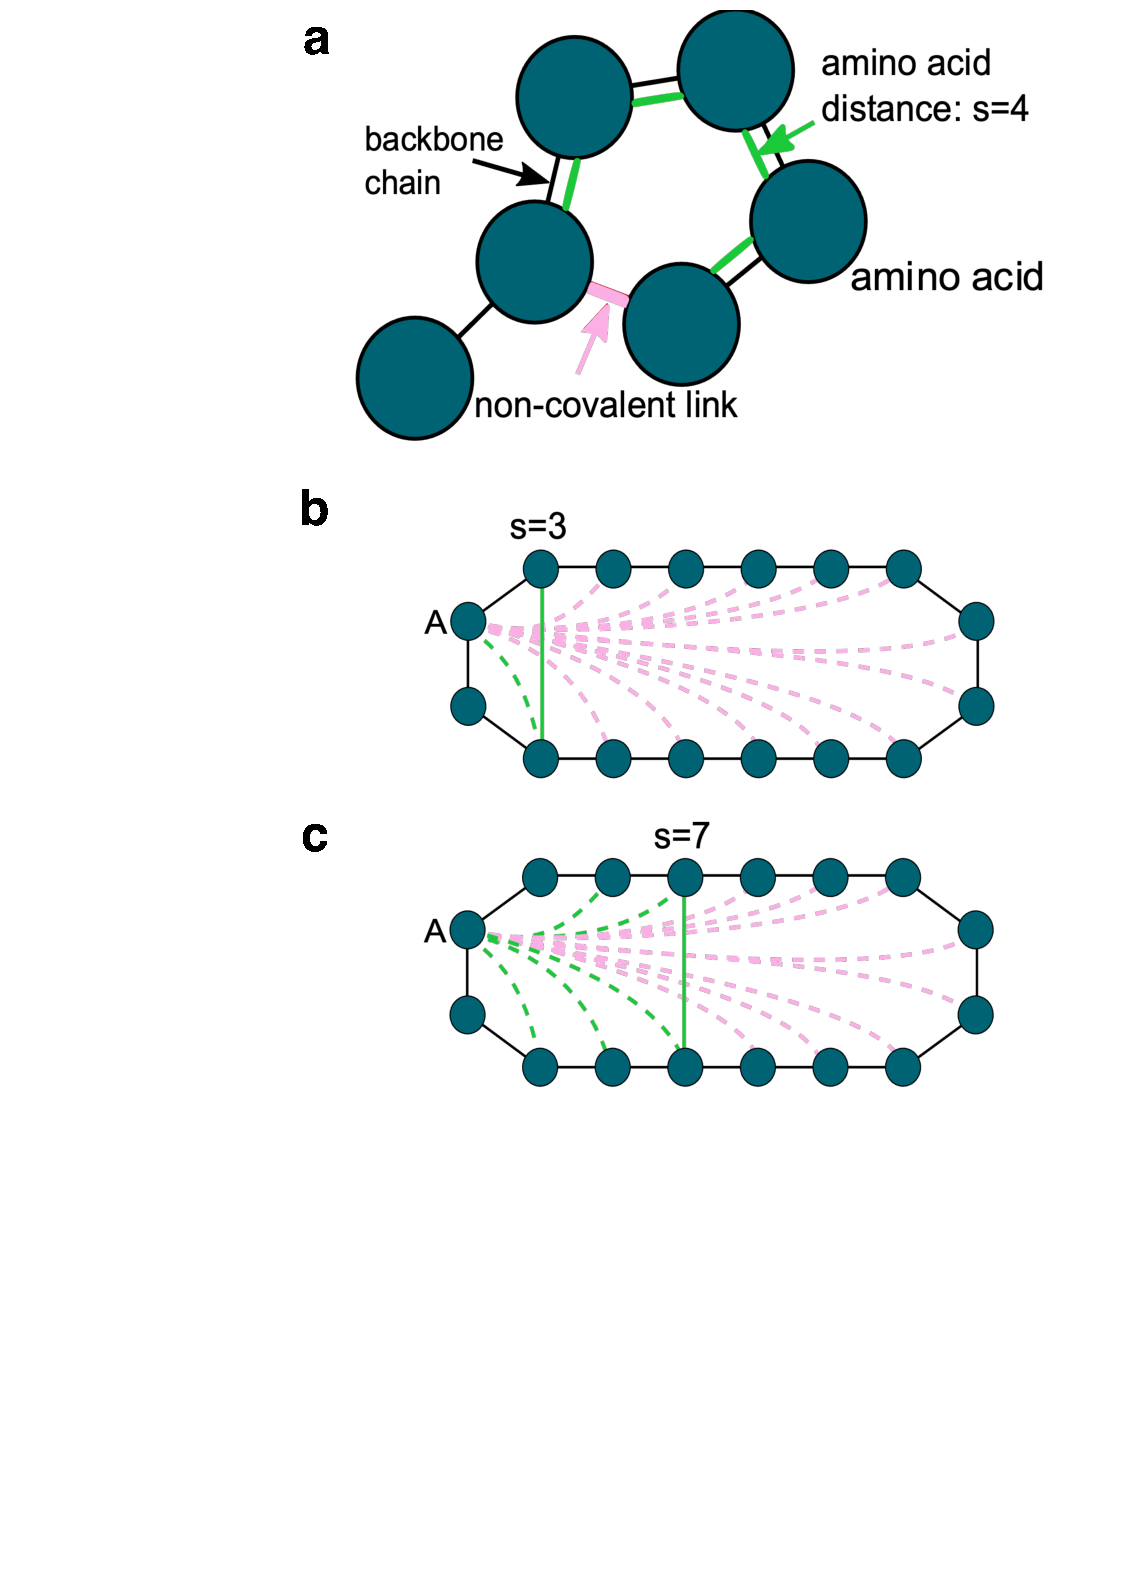
\includegraphics[width=0.8\columnwidth]{figures/Fig1/Fig1.pdf}
    \caption{a) The amino acid distance $s$ is defined as the separation along the chain (teal) of two connected units (pink). b)~The solid green link prohibits some connections from node~$A$ (dotted pink), while others are still permitted (dotted green). Counting all newly excluded links, we find that a link of length $s$ prohibits $2(l-1)$ links of length $l$ up to a maximum of $s$ and $2(s-1)$ links of length $s$ or more.}
    \label{fig:schematic}
\end{figure}

%%%%%%%%%%%%
% subsection
%%%%%%%%%%%%
\subsection{Contact maps in a geometrically constrained protein model}

Based on the basic observation that amino acids are objects in space which cannot overlap indefinitely, we introduced a model in~\cite{molkenthin2020self} starting from a chain of identical spheres, each in contact only with the neighbours it is connected to. Then additional connections form by randomly selecting two spheres and moving them towards each other until they touch, the new links formed that way can not be broken in later steps and function as constraints on subsequent links. If contact of the two selected spheres is geometrically impossible without breaking previously made connections or leading to overlaps of any spheres, the link is not made and taken out of the pool of possible connections. This process is repeated until no more links can be formed without violating the geometric constraints and the final structure can be expressed as the adjacency matrix
\begin{equation}
  \mathbf{A}^{\mathrm{sim}}_{ij}=
  \begin{cases}
   1, & \text{ if }|i-j|=1 \text{ or i and j  randomly connected} \\
      0, & \text{ otherwise }  .
      \end{cases}
    \label{eq:aij}
\end{equation}

In~\cite{molkenthin2016scaling}, we have introduced a simplified, two-dimensional version of this model, which starts from a closed chain (i.e. a ring) of $N$ unit discs and subsequently adds links, such that connected discs touch, yet no discs intersect. The advantage of this model is that it can be approximated by a purely topological simplification, which can be treated analytically. Fig.~\ref{fig:schematic} illustrates the construction of the 2D geometric model.




The topological constraints in the resulting network model are:
(a) New links always form between two units that are part of the same face of the graph (region enclosed by a cycle in the network). This prevents the overlapping of discs. (b) No links form across the outer face. This prevents the enclosure of a unit by less than six other units (which is geometrically impossible) such that (c) the maximum degree of each unit is six, as six is the maximum number of unit discs one central unit disc can touch. (d) Once connected by a link, pairs of units do not disconnect.

%%%%Missing%%%%%
% TO DO: @Nora
% Describe how the protein contact maps are generated in the geometric constrained model %
% Let's call the adjacency matrix in this case \mathbf{A}^{\mathrm{sim}}_{ij} where sim stands for simulation. 
%%%%%%%%%%%%%%%

\subsection{Protein contact maps from structural protein data}

The underlying formation mechanisms of individual protein folds are incredibly complex and depend on the surrounding solvent, as well as the specific amino acid sequence and their quantum-mechanical interactions. Here we want to assess if the geometrically constrained protein model's contact map distributions capture real protein behavior as suggested in~\cite{bartoli2008effecta}. To understand this better, we want to study the ensemble of PCMs from real protein structures. To this end we will look at `averaged' contact maps over many different proteins that have different amino acid sequences, but their overall sequence or chain length is the same. 
We will use the RCSB protein data bank (PDB), a database of structurally resolved protein amino acid sequences through X-ray crystallography, NMR or cryo-EM experiments and the synthetically generated structural database from the machine learned structures of AlphaFold~2~\cite{jumper2021highly}. The PDB contains just under 200,000 protein structures to date~\cite{PDB}. The distribution of amino acid chain lengths in the PDB is illustrated in Fig.~\ref{fig:pdb_stats} b. Protein chain lengths in the PDB vary from small fragments of less than 10 amino acids to large agglomerates of over 2000 amino acids. The most frequently occurring chain lengths, however, are between 100 and 300 amino acids as shown in Fig.~\ref{fig:pdb_stats} b. The pink subset of the barplot shown in Fig.~\ref{fig:pdb_stats} b, are the set of structures used that fulfill the criterion on amino acid chain lengths between 85 and 115 amino acids, 185 and 215 amino acids and 285 and 315 amino acids and represent all structures for the analysis. The second database consists of synthetically generated structures using AlphaFold~2 with sequences taken from SwissProt~\cite{alpha fold 2 database}. SwissProt is a manually curated database of protein sequences containing over 500,000 protein sequences~\cite{SwissProt}, whose amino acid chain length distribution is shown in Fig.~\ref{fig:pdb_stats} a in teal. The pink bars again indicate the subset of AlphaFold~2 structures used for the contact map analysis. In this case, the used structures were filtered first with the condition that the AlphaFold~2 pre-residue confidence score~\cite{jumper2021highly} was `Very high', i.e. above 90 out of 100, and then by removing any structures describing the same protein to remove duplicates.

 \begin{figure}[t]
        \centering
	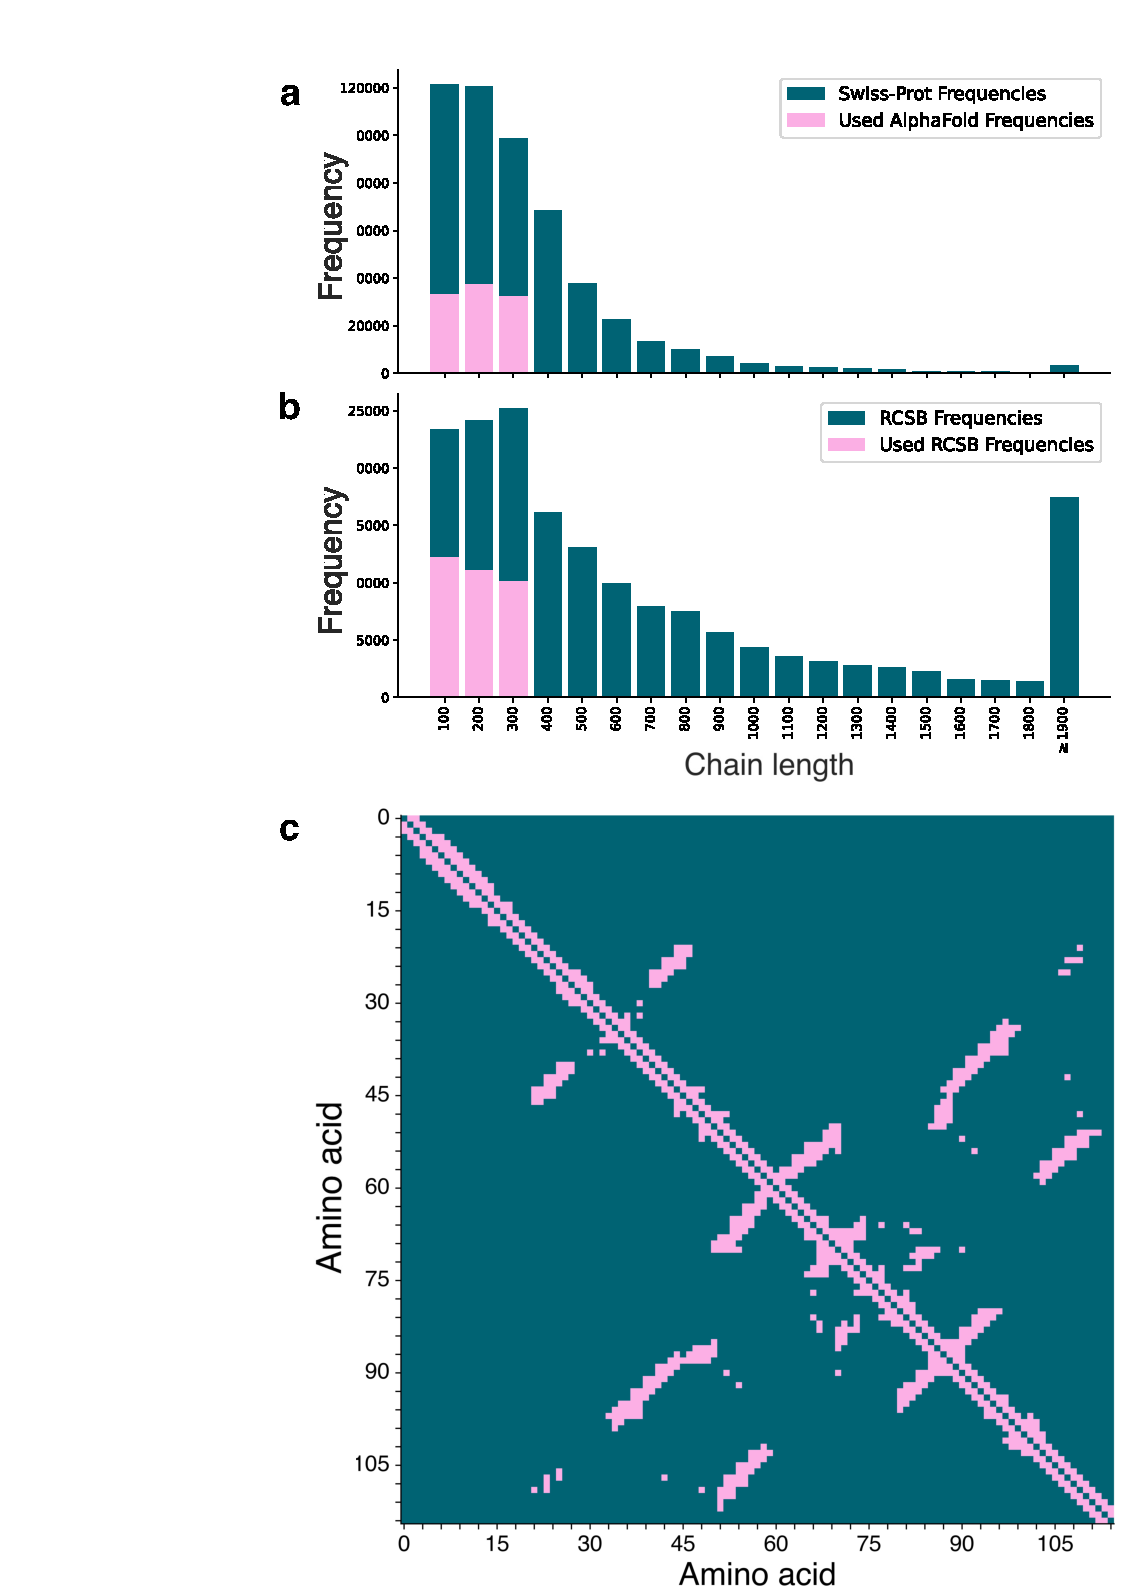
\includegraphics[width=0.8\columnwidth]{paper/figures/Fig2/Fig2.pdf}
	    \caption{Histogram of protein sequence lengths for protein structures from two structure databases. a) AlphaFold~2~\cite{jumper2021highly} predicted protein structures taken from protein sequences in the reviewed Uniprot Knowledge Base (Swiss-Prot) database based on their Uniprot IDs. Pink bars show fraction of structures used for the average contact map analysis.  b) RSCB~\cite{PDB} PDB chain length frequencies based on sequence length. Pink bars in plot show protein structures whose sequence lengths matches the resolution of structure accounting for the whole sequence. Only pink PDB samples were used for the average contact map analysis. c) Example of a protein contact map taken from PDB ID: 3UFG, with a cut-off of 8~Å. Pink squares indicate a contact present between amino acids.}
        \label{fig:pdb_stats}
\end{figure}
All structure-based contact maps are generated in the same way for AlphaFold~2 structures and PDB structures. Structures used were downloaded in pdb format, read in with MDAnalysis version 2.0.0~\cite{gowers2016mdanalysis} and only C$_{\alpha}$ were selected and used for the analysis. Proteins were categorised by length and placed into three groups. Amino acid chain lengths between 85 and 115 amino acids, 185-215 amino acids and 285-315. For each of the used sequences, all pairwise C$_{\alpha}$ distances were assessed and two C$_{\alpha}$ atoms were in contact if their distance was less than 8~Å. All pairwise distances were evaluated and in this way, building up the binary contact map or adjacency $A_{ij}^{\mathrm{struc}}$.  
All code for the construction of the contact maps both for the geometrically constrained system and structural protein data and their analysis can be found on GitHub at: \url{https://github.com/meyresearch/sequence_distance_distribution}.


%%%%%%%%%%%%
% Section. %
%%%%%%%%%%%%
\section{Analytic approximation for the geometrically constrained model}

To assess how we can best describe the distribution of the probability of amino acid distances as obtained by a PCM for the geometrically constrained model, we propose the following analytical approximation. To be able to do this we will look at the amino acid distance distribution for the simplified 2D model. Fig~\ref{fig:schematic} summarizes the idea behind this two-dimensional model.

Let us start by introducing the auxiliary variable $F_k(s)$, defined to be the number of possible links with an amino acid distance of $s$ if $k$ links have been added before. Before any links are added, all amino acid distances are equally likely, as there are $F_0(s)=N$ possibilities of making a link of each distance $s$ with $2\leq s < \frac{N}{2}$.

As we add more links, not only are links taken out of this pool, because they have already been realized, \red{but} each existing link can also geometrically prohibit other connections. Adding a link of length $s_1$ prohibits $2(s-1)$ links of length $s<s_1$ and $2(s_1-1)$ links of length $s>s_1$ (see Fig.~\ref{fig:schematic}~b). To find the expected number of links still available in subsequent steps, we average over all possible amino acid distances $s_1$ of the first link added.

The expected distribution of possible links after one step is \red{thus given} by the average over available link pools taken over all possible values of $s_1$
\begin{equation}
\begin{aligned}
    F_1(s)&=\frac{1}{N/2-1} \sum_{s_1=2}^{N/2}{ \begin{cases}
    F_0(s)-2(s-1) \text{ , for } s<s_1\\
    F_0(s)-2(s_1 -1)\text{ , for } s\geq s_1
    \end{cases}}
    \nonumber \\
    &\approx\frac{2}{N} \sum_{s_1=2}^{N/2} { \begin{cases}
    N-2(s-1) \text{ , for } s<s_1\\
    N-2(s_1 -1)\text{ , for } s\geq s_1
    \end{cases}}
\end{aligned}
    \label{eq:reduction_first_step}
\end{equation}

After $k-1$ links were made, the probability that the $k$-th link, being randomly chosen from the pool of available links, has length $s$ obeys
\begin{equation}
    \Pin^k(s)=F_k(s)/C_k,
\end{equation}
where $C_k=\sum_{s=2}^{N/2}F_k(s)$. In subsequent steps, we use this probability to perform a weighted average over new links being added, and get the same reduction (compare Fig.~\ref{fig:schematic}) but starting from the pool $F_{k-1}(s)$ of the step before rather than the initially available $N$ links. However, we must subtract fewer links to account for some of them having left the pool in earlier steps. To this end, we multiply the number of blocked links by
\begin{equation}
    \frac{F_{k-1}(s)}{F_0(s)} = F_{k-1}(s)\frac{1}{N}.
    \label{eq.Pk}
\end{equation}
% \begin{equation}
%     P_k(s)=\frac{F_k(s)}{C_k},
%     \label{eq.Pk}
% \end{equation}
%with $C_k=\sum_{s=2}^{N/2}F_k(s)$, 
This ignores any length-dependent bias in which links have been removed, however, examples suggest this assumption seemed to hold well. 
This leads to the recursion
\begin{align}
    F_k(s)&= \sum_{s_k=2}^{N/2} \Pin^k(s_k)\nonumber \\
    & \left(F_{k-1}(s)-  F_{k-1}(s)\frac{1}{N}
    {\begin{cases}
     2(s-1) \text{ , for } s<s_k\\
     2(s_k -1))\text{ , for } s\geq s_k
    \end{cases}} \right)
\end{align}
which generalizes equation~\ref{eq:reduction_first_step} and simplifies to
\begin{align}
   F_k(s)&=F_{k-1}(s)(1-\frac{1}{N} \sum_{s_k=2}^{s} (2 (s_k-1) \Pin^k(s_k))\nonumber \\
   &-\frac{1}{N} \sum_{s_k=s+1}^{N/2} (2 (s-1) \Pin^k(s_k)))\nonumber \\
   &=F_{k-1}(s)(1-\frac{1}{N}
   \sum_{s_k=2}^{s} (2 (s_k-1) \Pin^k(s_k))\nonumber \\
   &-\frac{2 (s-1)}{N} (\sum_{s_k=2}^{N/2} \Pin^k(s_k) - \sum_{s_k=2}^{s} \Pin^k(s_k)))\nonumber \\
   &=F_{k-1}(s)(1-\frac{2}{N} (s-1) 
   +\frac{2}{N} s
   \sum_{s_k=2}^{s}\Pin^k(s_k)\nonumber \\
   &-\frac{2}{N}
   \sum_{s_k=2}^{s} s_k \Pin^k(s_k))
   \label{eq.Fk_rec}
\end{align}

Together with the initial condition $F_0(s)=N$, this expression constitutes an iteration rule from which $F_k(s)$ can be found for all $k$ and $s$. Aiming to decouple those dynamics for different $s$, we make a heuristic guess for $\Pin^k(s_k)$. It consists of two separate approximations which are used in steps $k<a$ and steps $k\geq a$ respectively, where the threshold $1\leq a\leq N/2$ is a free parameter. In the early stage we use a uniform probability
\begin{equation}
    \Pin^{k\ll N/2}(s)\approx \Pin^{k=0}(s)=\frac{2}{N}.
    \label{eq.P_small}
\end{equation}
For later steps, the probability of a link to still be in the pool decreases with $s$. We thus approximate $\Pin(s)$ with an ansatz for the $k-$average, namely, that it drops off as $\frac{1}{s}$, leading to
\begin{equation}
    \Pin^{k\gg 1}(s)\approx \sum_{k=a}^{N-4}\Pin^{k}(s)
    \approx \frac{s^{-1}}{ (H_{\frac{N}{2}}-1)},
    \label{eq.P_large}
\end{equation}
where $H_{\frac{N}{2}}$ is the harmonic number serving as a normalization factor. 
As we will see later this approximation holds most precisely for intermediate values of $k$, with the $k-$average of $\Pin^{k\gg 1}(s)\approx P(s)$, making it self-consistent. Errors for smaller and larger values of $k$ are thought to approximately cancel out.
Substituting Eq.~\ref{eq.P_small} and Eq.~\ref{eq.P_large} into Eq.~\ref{eq.Fk_rec} results in the following two recursions for the early and late evolution of the amino acid distance distribution respectively.
\begin{align}
   F_{k\ll N/2}(s)&\approx 
   F_{k-1}(s)(1-\frac{2}{N} (s-1) 
   +\frac{4}{N^2} s (s-1)\nonumber \\
   &-\frac{2}{N^2}(s^2+s-2)\nonumber \\
   &=F_{k-1}(s)(1-\flow(s)),
   \label{eq.Fk_rec_low}
\end{align}
where 
\[\flow(s)=-\frac{2}{N^2}s^2+\left(\frac{2}{N}+\frac{6}{N^2}\right)s-\left(\frac{2}{N}+\frac{4}{N^2}\right),\]
and


\begin{align}
   F_{k\gg1}(s)&\approx 
   F_{k-1}(s)(1-\frac{2}{N} (s-1) 
   +\frac{2}{N} s \sum_{s_k=2}^{s}\frac{1}{s_k(H_{\frac{N}{2}}-1)}\nonumber\\
   &-\frac{2}{N}
   \sum_{s_k=2}^{s} s_k \frac{1}{s_k(H_{\frac{N}{2}}-1)})\nonumber \\
   &=
   F_{k-1}(s)(1 -(\frac{2}{N}-\frac{2}{N}\frac{H_{s}-1}{H_{\frac{N}{2}}-1}+\frac{2}{N(H_{\frac{N}{2}}-1)})s \nonumber \\ 
   &+ \frac{2}{N(H_{\frac{N}{2}}-1)} + \frac{2}{N})\nonumber \\
   &=F_{k-1}(s)(1-\fhigh(s)).
   \label{eq.Fk_rec_high}
\end{align}
where 
\[\fhigh(s)=\frac{2}{N}(\frac{H_{\frac{N}{2}}-H_{s}+1}{H_{\frac{N}{2}}-1}s-\frac{H_{\frac{N}{2}}}{H_{\frac{N}{2}}-1}).\]

We can now use the recursive expressions to write down a closed expression for $F_k(s)$, using $\flow$ for the first $a$ steps and $\fhigh$ for the rest:

\begin{align}
    F_k(s)&=N\prod_{i_1}^a\left(1-\flow(s)\right)\prod_{i=a+1}^k\left(1-\fhigh(s)\right) \nonumber \\
    &= N\left(\frac{1-\flow(s)}{1-\fhigh(s)}\right)^a\left(1-\fhigh(s)\right)^{k}
\end{align}

In 2D this is repeated for $N-3$ steps until no more links can be added \cite{molkenthin2016scaling}.
The probability distribution of the realized amino acid distances of all added links is then given by the average over the available pools at each link addition step, leading to
\begin{align}
    P(s)&=\frac{1}{N-3}\sum_{k=0}^{N-4} \frac{F_k(s)}{C_k} \nonumber \\
    &\approx \frac{N}{N-3}\left(\frac{1-\flow(s)}{1-\fhigh(s)}\right)^a
\sum_{k=0}^{N-4} \frac{1}{\evdel{C_k}_k} \left(1-\fhigh(s)\right)^{k} \nonumber \\
    &\approx \left(\frac{1-\flow(s)}{1-\fhigh(s)}\right)^a\frac{A}{\fhigh(s)},
    \label{eq.Ps}
\end{align}
where $\evdel{C_k}_k$ is the average of $C_k$ over $k$.
This approximation allows the use of the geometric series for solving the equation. 
The resulting expression in Eq.~\ref{eq.Ps} is by visual inspection of Fig.\ref{fig:2d_sim} resembles a power law with an exponent of -1, thus justifying the earlier approximation of $\Pin^k(s)$.
%which makes use of Eq.~\ref{eq.Pk}. 
%The only unknown in this expression is $C_k$, \red{which we can not compute exactly...?}. However, since $C_k$ monotonically decreases with $k$, $N>C_k>C_{N-2}$ always holds and we can obtain an upper and lower bound by replacing all $C_k$ in the expression with either $N$ (underestimates all probabilities) or $C_{N-2}$ (overestimates all probabilities). Each time we get an expression of the form 
% \begin{align}
%      P(s)&\approx\frac{N}{N-3}\sum_{k=0}^{N-3} \frac{1}{C_k}\prod_{i}^k\left(1-\frac{f(s)}{(\frac{N}{2}-2)C} \right)\nonumber \\
%      &=\frac{N}{N-3} \sum_{k=0}^{N-3}\frac{1}{C_k}\left(1-\frac{f(s)}{(\frac{N}{2}-2)C} \right)^k \nonumber \\
%      &\approx \frac{A}{f(s)}
% \end{align}
% for $1<s<\frac{N}{2}$,
% where $A$ is an unknown constant, containing an approximation of the various normalization constants $C_i$, as well as the direct effects of the chain length. 

%In the last step of this approximation, we took the $C_k$ to all be approximately equal in order to apply the geometric series. However, in reality we know $1/C_k$ to increase with $k$, giving large $k$ summands relatively more weight than in a geometric series. This can be expressed as a small correction $\alpha$ in the exponent.



\section{Results}
\subsection{Analytic approximation and 2D simulations}
Fig.~\ref{fig:2d_sim} compares Eq.~\ref{eq.Ps} with respect to the two-dimensional (a) and three-dimensional (b) simulation data introduced in~\cite{molkenthin2020self}. The 2D simulation data, generated from 10 repeats with chain lengths of up to 498 amino acids, consists of frequencies of amino acid distances in each simulation run, while the 3D simulation data consists of adjacency matrices computed from 30 simulation runs, and was analyzed the same way as the PDB and AlphaFold~2 protein data. These are plotted showing the mean frequencies of each amino acid distance up to $\frac{N}{2}\sim250$ and $\frac{N}{2}\sim150$ for 2D and 3D simulations, respectively. The shaded areas represent the 95\% confidence intervals. The theoretical approximation from Eq.~\ref{eq.Ps} was fitted to both the 2D and 3D simulation data separately. The two parameters, the exponent $a$, and the dimensionality constant $A$, were given by the fit as $a_{\mathrm{2D}}=6 \pm 1$, $A_{\mathrm{2D}}=(3.0 \pm 0.5)\cdot 10^{-4}$ and $a_{\mathrm{3D}}=1 \pm 1$, $A_{\mathrm{3D}}=(7 \pm 2)\cdot 10^{-3}$ for 2D and 3D simulations, respectively. The fitted approximation captures the behavior of the simulation data well, as in the case for 2D simulations, both describe two-dimensional systems.

 \begin{figure}[htb]
        \centering
	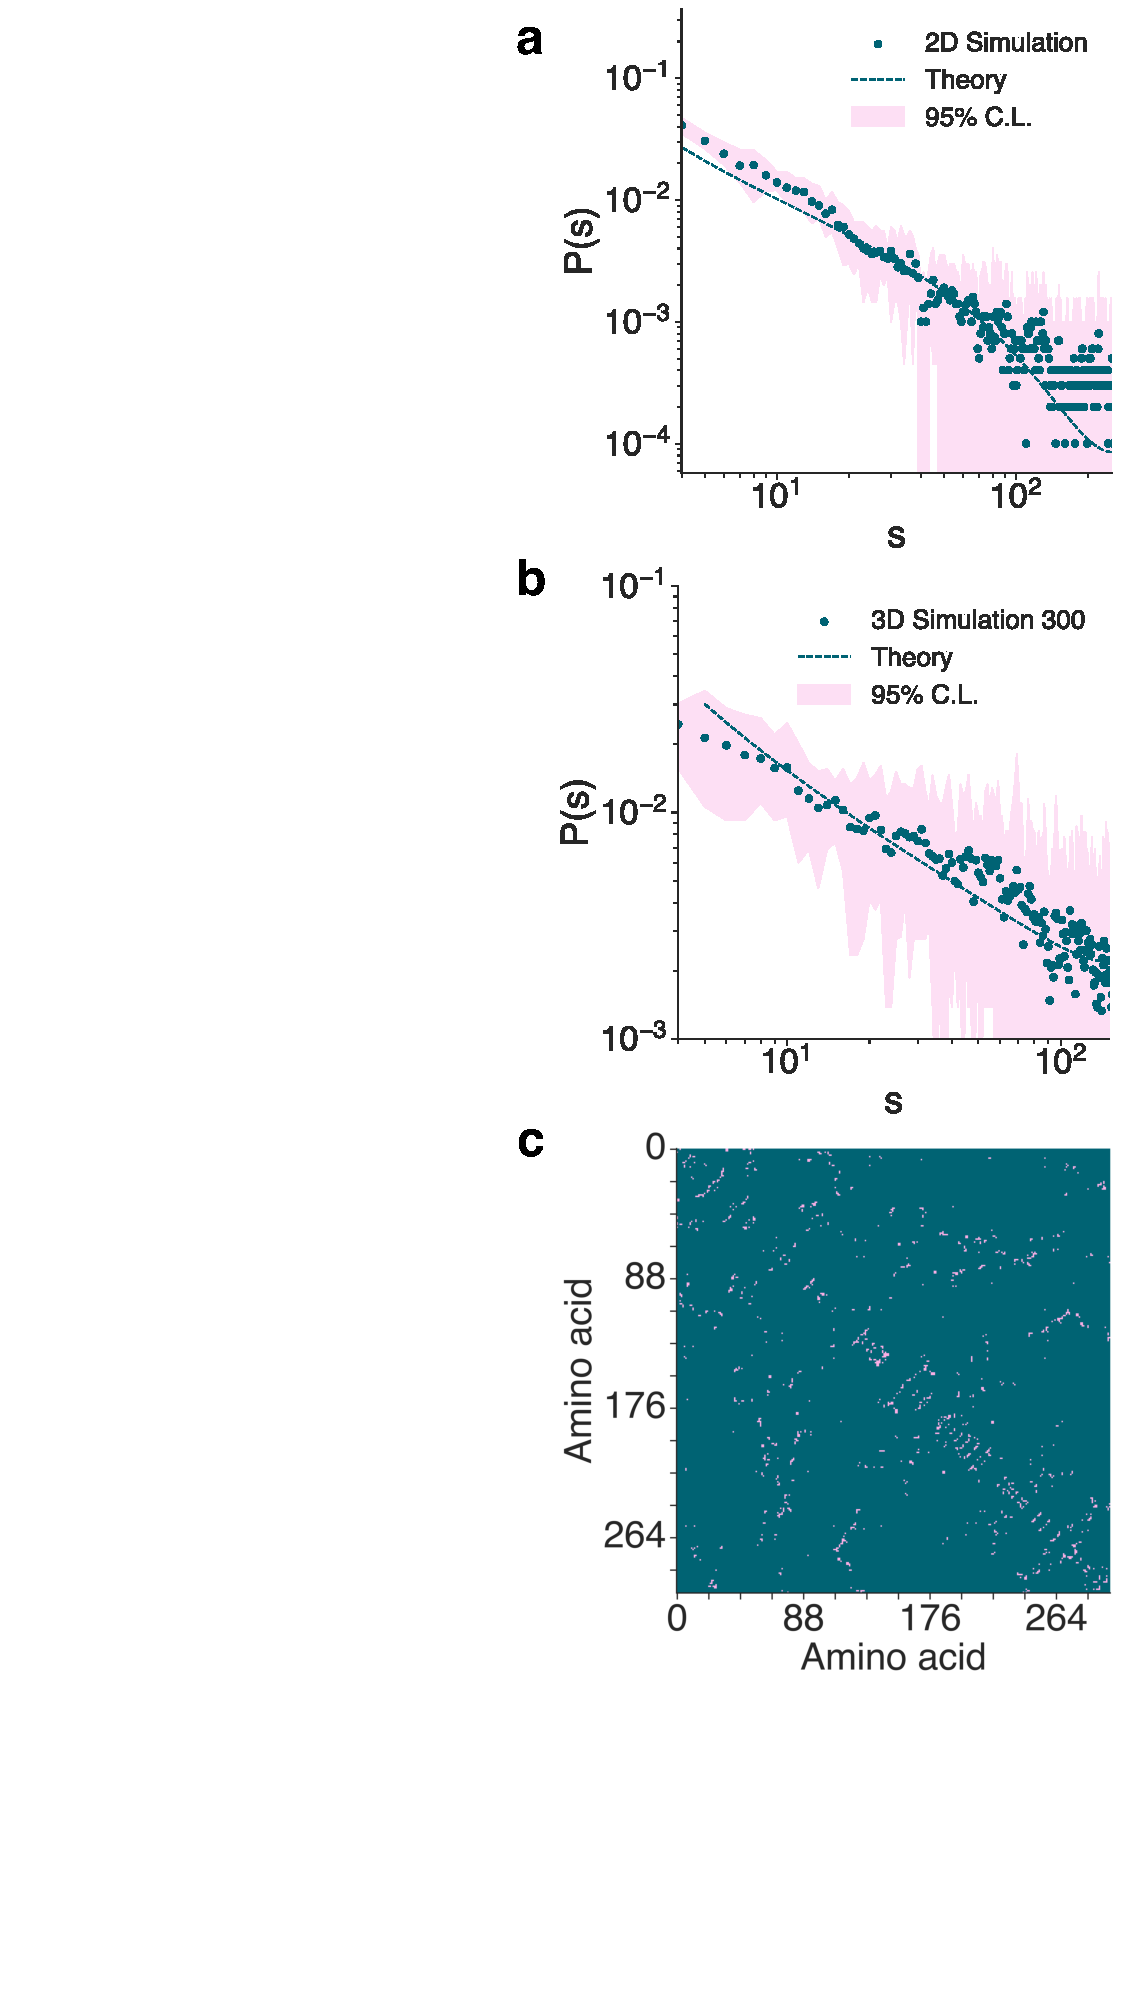
\includegraphics[width=\columnwidth]{paper/figures/Fig3/Fig3.pdf}
	    \caption{Amino acid distance distributions for a) two-dimensional and b) three-dimensional simulated data plotted against the analytic approximation. Pink area shows the 95\% confidence interval. c) Example of a protein contact map taken from one of the three-dimensional simulation runs. The pink squares indicate a contact between two nodes.}
        \label{fig:2d_sim}
\end{figure}

\subsection{3D simulations and PCMs from structural data }
%Next, we investigate if and how the analytical approximation can also capture trends in 3D simulation data, as well as experimentally determined protein structures. 
Next, we investigate if and how the analytical approximation can also capture trends in the experimentally determined protein structures.
This seeks to answer the question if indeed a power law can be used to describe the probability distribution of amino acid distances. We have chosen a subset of structures from the RCSB~\cite{PDB} and AlphaFold~2~\cite{jumper2021highly} databases for the analysis. From the RCSB database, 12,206 structures with chain lengths that fall between 85-115, 11,031 structures that fall between 185-215, and 10,091 structures that fall between 285-315 amino acids were selected. Additionally, 17,370 structures with chain lengths in the range of 85-115, 24,665 in the range of 185-215 and 21,804 in the range of 285-315 amino acids were chosen from the AlphaFold~2 database~\cite{jumper2021highly}. All structures were converted into PCMs as described in Section~\ref{sec:methods}. 

Fig.~\ref{fig:sdd} a summarises the results for protein chain lengths of $\approx100$, $\approx200$ and $\approx300$ amino acids, most commonly found in living organisms (see Fig.~\ref{fig:pdb_stats} a). This also shows how the amino acid distribution is scaled with respect to increasing chain lengths.

In Fig.~\ref{fig:sdd} b, we compare data from  protein contact maps from RCSB~\cite{PDB}, and AlphaFold~2~\cite{jumper2021highly} for protein chain lengths of $\approx300$ amino acids. The resulting distributions for each chain length interval are plotted logarithmically scaled in Fig.\ref{fig:sdd} a for intervals 85-115 (100), 185-215 (200), and 285-315 (300). For all three lengths, the distributions show an approximate power law decay, for both the 3-D simulations according to~\cite{molkenthin2020self}, as well as the structural data. This allows a fit  which is consistent with both the simulated results and the theoretical approximation. We also fit the analytic approximation as well as a general power law to the RCSB structures in this range. The shaded area shows the 95\% confidence level (C.L.). The parameters given by the theoretical approximation are $a=4 \pm 1$ and $A=(7.4 \pm 0.8)\cdot 10^{-4}$. As for the power law, the exponent is $\gamma=1.44 \pm 0.02$, meaning that this is a scale-free network ($1\leq\gamma\leq2$). We also analyze the amino acid distributions from the chosen RCSB and AlphaFold~2 structures by calculating the Kolmogorov-Smirnov (KS) statistic. The KS statistic for the protein chain lengths of $\approx$300 amino acids was 0.12 and thus the null hypothesis was accepted at the $\alpha=0.01$ level.
%Fig.~\ref{fig:sdd} summarises the results for protein chain lengths of $\approx$100 (a), $\approx$200, and $\approx$ 300 amino acids, protein chain lengths, most commonly found in living organism (see. Fig.~\ref{fig:pdb_stats} a). 
%We are comparing data from repeats of 30 simulation runs of the three-dimensional simulations, as introduced in~\cite{molkenthin2020self}, and protein contact maps from RCSB~\cite{}, and AlphaFold~2~\cite{}. 

\begin{figure}[h!]
        \centering
	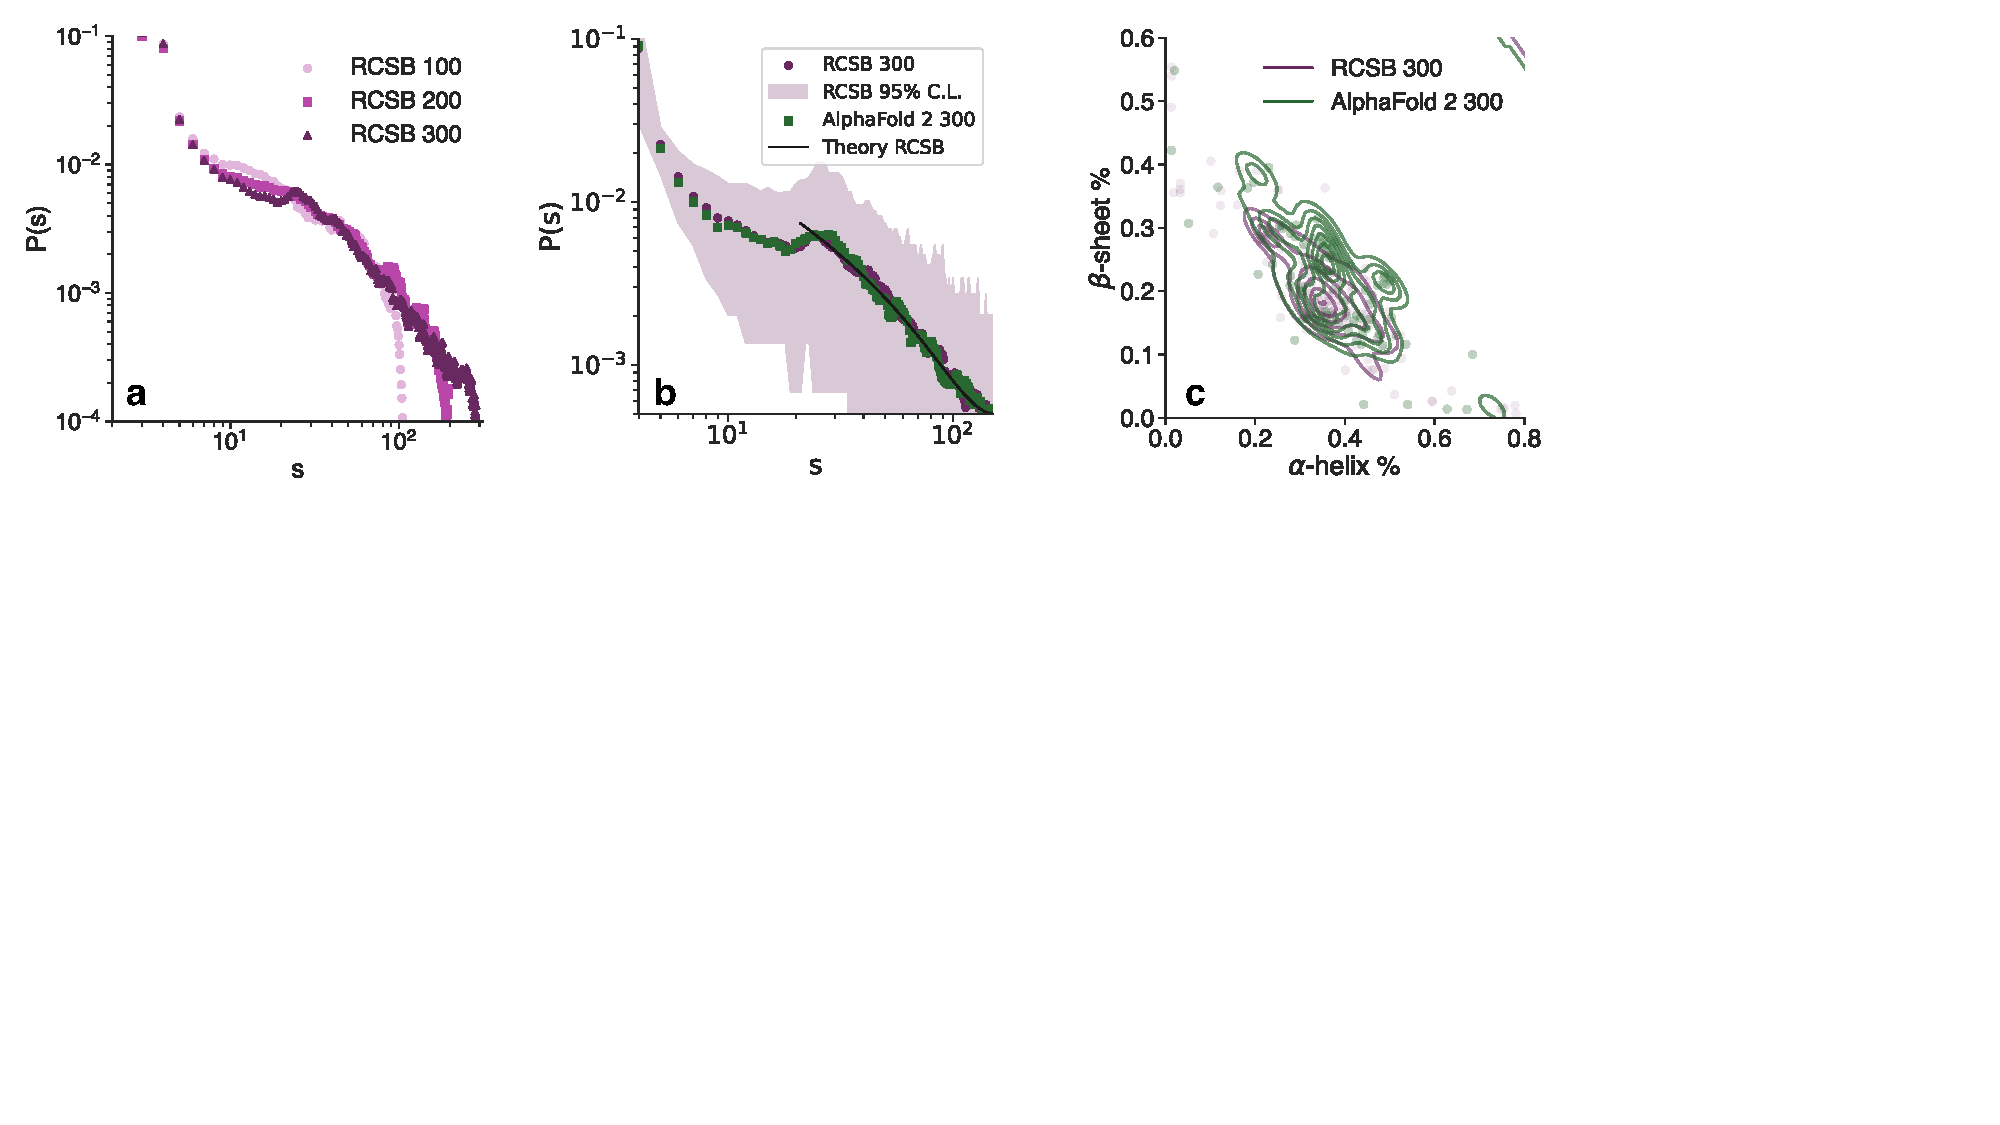
\includegraphics[width=\columnwidth]{paper/figures/Fig4/Fig4.pdf}
        \caption{a) Amino acid distance distributions for contact maps derived from the RCSB~\cite{PDB} database for protein chains in the ranges of 85-115 (100), 185-215 (200) and 285-315 (300) amino acids. b) Comparison between the distributions of RCSB~\cite{PDB} and AlphaFold~2~\cite{jumper2021highly} databases for protein chains in the $\approx300$ range. The analytic approximation (solid line) and power law (dashed line) are fitted to the tail of the RCSB data. Pink shaded area shows the 95\% confidence level. c) Secondary structure content distribution in the RCSB~\cite{PDB} and AlphaFold~2~\cite{jumper2021highly} structures in the $\approx300$ chain length range.}
        \label{fig:sdd}
\end{figure}

Finally, Fig.~\ref{fig:sdd} c shows the secondary structure content distributions for proteins in the $\approx300$ chain length range from RCSB and AlphaFold~2. This shows us that the proteins in this range seem to mostly contain secondary structures in the combined $\alpha$-helix---$\beta$-sheet region. Similar plots for the protein chain length regions of $\approx100$ and $\approx200$ amino acids can be found in the Supplementary Materials.


%is compared to those generated in simulations in~\cite{molkenthin2020self} as well as the above derived theoretical expression scaled with a factor to account for the different dimensionality, i.e. constant $A$, as well as approximations made in the derivation.

%For large values of the chain length $N$, we thus find an approximate power law probability distribution for the amino acid distance with an exponent of $-1+\alpha$. 

We observe that, while the general shape seems to match, in real proteins amino acid distances of two to four amino acids are slightly over-represented (see Fig.\ref{fig:sdd} a and b).
The over-representation of very short amino acid distances is an artefact of the different network construction for simulated (and theoretically approximated) networks and PCMs. While in the simulation all links are equally long and links are made until no longer possible, the parameter, determining the connectivity in PCMs is the cutoff distance $d_c$\blue{(mention used value?)}, which is chosen such that the number of links in the PCM is comparable to those in a simulated network of the same $N$. This leads to a larger range of bond angles randomly resulting in connections for small $s$ and thus an over-representation of those links.


%Here we use 30 runs of three-dimensional simulations, as introduced in~\cite{molkenthin2020self}, and networks extracted from measured protein data from both the RCSB~\cite{PDB} and AlphaFold~2~\cite{} databases to compare this behavior with the more realistic 3D settings and 

\red{...show that the basic principle persists, indicating that much of the amino acid distance distribution can be attributed to generic geometric constraints.}

\section{Conclusion}
The tertiary structures of folded proteins have long been one of the most important mysteries of Biophysics. While for individual structures, detailed molecular dynamics or statistical models are essential in approaching these questions, general statements for the ensemble of folded proteins can be made with simple models.

Here we have introduced and analyzed the amino acid distance $s$ and its probability distribution $P(s)$ in measured and simulated protein structures. For the equivalent model in two dimensions we have used a mean-field approach to derive an analytic approximation for the amino acid distance distribution, which appears to agree with the simulated and measured distributions.
We have thus demonstrated in analytical calculations as well as direct simulations how a random linking model with geometric constraints, such as the ones introduced in~\cite{molkenthin2016scaling, molkenthin2020self}, generates a amino acid distance distribution that resembles a power-law, similar to the one found in folded proteins. This feature of protein network structures has previously been used in a heuristic manner to model and generate protein-like structures in \cite{bartoli2008effecta}.

Gaining a better understanding of the ensemble of folded protein structures can help guide the way to a better understanding of the constraints within which structures may occur. Together with an understanding of secondary structure principles, such as those in
~\cite{Danielsson2010, Molkenthin2011}, this can help to narrow down the complex energy landscapes and find paths through them more effectively in the future.

\section*{Declarations}
\subsection{Availability of data and materials}
All data generated or analysed during this study are included in this published article. All raw data and their analysis can be found on GitHub at: \url{https://github.com/meyresearch/sequence_distance_distribution}, including information required for their reproduction. 
\subsection{Competing interests}
The authors declare no competing interests.
\subsection{Funding}
This research was supported by ...
\subsection{Authors' contributions}
N.M. and J.J.G. contributed equally to this work.
\subsection{Acknowledgements}
We thank Marc Timme, and Matteo Degiacomi for fruitful discussions.

\bibliographystyle{unsrt}
\bibliography{proteins}

\end{document}